\documentclass{beamer}
\usepackage[utf8]{inputenc}
\usepackage[russian]{babel}
\usepackage{graphicx}
\graphicspath{{}}
\DeclareGraphicsExtensions{.pdf,.png,.jpg}

\usetheme{Madrid}
\usecolortheme{default}

%------------------------------------------------------------
%This block of code defines the information to appear in the
%Title page
\title[Задача коммивояжёра] %optional
{Задача коммивояжёра}

\subtitle{Метод ветвей и границ}

\author[Данила Печенев] % (optional)
{Данила~Печенев}

\institute[] % (optional)
{
  Программмная инженерия\\
  Математико-механический факультет\\
  СПбГУ
}

\date[Май 2022] % (optional)
{Май 2022}

%End of title page configuration block
%------------------------------------------------------------


\begin{document}

%The next statement creates the title page.
\frame{\titlepage}


%---------------------------------------------------------
%This block of code is for the table of contents after
%the title page
\begin{frame}
\frametitle{Содержание}
\tableofcontents
\end{frame}
%---------------------------------------------------------


\section{Формулировка задачи}

%---------------------------------------------------------
% Changing visivility of the text
\begin{frame}
\frametitle{Формулировка задачи}
В 19-м и 20-м веке по городам ездили коммивояжёры (сейчас их называют «торговые представители»). Они ходили по домам и предлагали людям купить разные товары. Тактика была такой: коммивояжёр приезжал в город, обходил большинство домов и отправлялся в следующий город. Города были небольшими, поэтому обойти всё было вполне реально.

Чем больше городов посетит коммивояжёр, тем больше домов он сможет обойти и больше заработать с продаж. Самая большая проблема, которая всегда стояла перед коммивояжёрами, звучала так:

\begin{center}
  Как быстрее всего объехать все города в этом районе?
\end{center}

\end{frame}


\begin{frame}
\frametitle{Формулировка задачи}
В 19-м веке все добирались из города в город на лошадях и повозках, поэтому время полностью зависело от расстояния между городами. С другой стороны, коммивояжёру нужно было вернуться домой после поездок, поэтому \textbf{классическая задача коммивояжёра} звучит так:

\begin{center}
\textbf{Как найти самый короткий маршрут между городами, чтобы побывать в каждом хотя бы по одному разу и вернуться домой?}
\end{center}
\end{frame}

%---------------------------------------------------------

\section{Формальнее: математическая модель}

%---------------------------------------------------------
\begin{frame}
\frametitle{Формальнее: математическая модель}
Задан полный ориентированный граф $G = (V, E)$ с множеством вершин $V = \{1, …, n\}$ и множеством дуг $E$. Каждой дуге $(i, j) \in E$ сопоставляется
длина $c_{ij} \geq 0$. В общем случае задача коммивояжёра формулируется на
произвольном графе, поэтому длины некоторых (в частности, не существующих) ребер могут быть сколь угодно большими. Будем считать, что
$c_{ii} = +\infty$ (тем самым указываем на бессмысленность перемещения из города $i$ в этот же город $i$).\\
Таким образом, требуется найти гамильтонов цикл $(i_1, i_2, \ldots, i_n, i_1)$ минимальной длины, где $i_k$ - номер $k$-го посещенного города.

\end{frame}

% In this slide, some important text will be
% \alert{highlighted} because it's important.
% Please, don't abuse it.

% \begin{block}{Remark}
% Sample text
% \end{block}

% \begin{alertblock}{Important theorem}
% Sample text in red box
% \end{alertblock}

% \begin{examples}
% Sample text in green box. The title of the block is ``Examples".
% \end{examples}

%---------------------------------------------------------

\section{Метод ветвей и границ}

%---------------------------------------------------------

\begin{frame}
\frametitle{Метод ветвей и границ}
Пусть задана таблица $C$ длин дуг из множества $E$. Расстояние между вершинами $i$ и $j$, как и ранее, обозначаем за $c_{ij}$ (соответствующая ячейка таблицы $C$). Опишем метод ветвей и границ для решения задачи коммивояжёра.\\
\textbf{Шаг 0:} Обозначим $c_{ii} = +\infty,\,i = 1, \ldots, n$.\\
\textbf{Шаг 1:} Рассмотрим произвольный путь и посчитаем его длину. Это будет верхняя граница длины пути. Далее, если в какой-то момент мы получим нижнюю оценку на длину пути большую, чем это число, мы тут же перестанем рассматривать этот вариант.\\
\end{frame}

\begin{frame}
\frametitle{Метод ветвей и границ}
\textbf{Шаг 2:} Редукция таблицы. Вычисляются $m_i' = min_jd_{ij},\,j = 1, \ldots, n$ - минимальные элементы в строках; $m_j'' = min_i(d_{ij} - m_i),\,i = 1, \ldots, n$ - минимальные элементы в столбцах после вычитания из $i$-ой строки $m_i,\,i = 1, \ldots, n$.\\
Производится редукция и получается новая таблица $C'$ в соответствии с формулой:
$$c_{ij}' = c_{ij} - m_i' - m_j'',\,1 \leq i,\,j \leq n.$$
Это преобразование основано на том факте, что при вычитании константы из любого столбца или строки матрицы стоимость оптимального маршрута уменьшится на величину этой константы, а маршрут останется тем же. 
\end{frame}


\begin{frame}
\frametitle{Метод ветвей и границ}
\textbf{Шаг 3:} Сумма всех вычтенных на предыдущем шаге величин и будет оценкой снизу для всех вариантов маршрута, построенных по матрице $C$. Вычислим нижнюю границу длины путешествия:
$$d = \sum\limits_{i=1}^n m_i' + \sum\limits_{j=1}^n m_j''.$$
\textbf{Шаг 4:} Ветвление. Производится выбор некоторого ребра графа, при котором все возможные варианты маршрута делятся на две группы: те, которые включают выбранное ребро, и те, в которых оно отсутствует. Для обеих групп создается отдельная матрица расстояний. Эти матрицы подвергаются аналогичному преобразованию с выбором ребра. Строящееся при этом дерево муршрутов получается бинарным.
\end{frame}

\begin{frame}
\frametitle{Метод ветвей и границ}
Выбор ребра на каждом шаге производится таким образом, чтобы оптимальный
вариант маршрута содержал выбранное ребро с наибольшей вероятностью. А именно, выбирается такое ребро $(i_0, j_0)$ с нулевым весом, для которого сумма весов вторых по минимальности ребер в его строке и в его столбце (иначе говоря, просматриваются все элементы, кроме текущего нулевого) максимальна.
Выбранное ребро включается в маршрут для вариантов маршрута первой группы и
исключается из всех вариантов маршрута второй группы.\\
\textbf{Шаг 5:} Вычисляется нижняя оценка длины пути для машрутов (узла в строящемся бинарном дереве), которые содержат ребро $(i_0, j_0)$. Раз это ребро точно есть в пути, то строку $i_0$ и столбец $j_0$ в $C'$ можно зачеркнуть (про них уже всё известно). С получившейся таблицей выполняются шаги 2 и 3.
\end{frame}

\begin{frame}
\frametitle{Метод ветвей и границ}
Далее вычисляется нижняя оценка длины пути для машрутов (узла в строящемся бинарном дереве), которые не содержат ребро $(i_0, j_0)$. В таблице $C'$ обозначается $c_{i_0j_0} = +\infty$ - это не позволяет коммивояжёру передвигаться из города $i_0$ в город $j_0$. Кроме того, все возможности закрытия цикла перед работой с матрицей в каждом узле дерева должны быть заблокированы (путем обозначения длин необходимых ребер, т.е. соответствующих ячеек таблицы, за $+\infty$).\\
\textbf{Шаг 6:} Из листов дерева выбирается тот, для которого нижняя оценка является наименьшей. С его таблицей выполняются шаги 2-6 и так далее.
\end{frame}

\begin{frame}
\frametitle{Метод ветвей и границ}
Алгоритм завершается, когда в таблице остаются только те маршруты, которые, если не
используются, приводят к решению, являющемуся траекторией бесконечной
продолжительности. В этом случае будет известна точная длина пути коммивояжёра. Все листы полученного бинарного дерева, нажняя оценка для которых больше, чем полученный результат, вычеркиваются. Остается проделать тот же алгоритм с оставшимися листами дерева, начиная с того, нижняя оценка которого минимальна. Наконец, среди всех полученных результатов выбирается путь с наименьшей длиной - такой путь и есть результат работы алгоритма. 
\end{frame}

%---------------------------------------------------------

\section{Пример: применение метода ветвей и границ на конкретной задаче}

%---------------------------------------------------------

\begin{frame}
\frametitle{Пример: применения метода ветвей и границ на конкретной задаче}
Рассмотрим пример применения метода ветвей и границ. Пусть задана следующая таблица расстояний между пятью городами (сразу выполним для нее шаг 0):
\begin{center}
$C=$
\begin{tabular}{ | l | l | l | l | l | l | }
\hline
& \textbf{1} & \textbf{2} & \textbf{3} & \textbf{4} & \textbf{5}\\ \hline
\textbf{1} & \infty & 10 & 25 & 25 & 10 \\ \hline
\textbf{2} & 1 & \infty & 10 & 15 & 2\\ \hline
\textbf{3} & 8 & 9 & \infty & 20 & 10\\ \hline
\textbf{4} & 14 & 10 & 24 & \infty & 15\\ \hline
\textbf{5} & 10 & 8 & 25 & 27 & \infty\\
\hline
\end{tabular}
\end{center}
Мы будем искать значение $F$ - наименьшую длину пути.\\
Шаг 1: рассмотрим какой-нибудь путь, например, $((1, 2), (2, 3), (3, 4), (4, 5), (5, 1))$. Несложно проверить, что его длина 65 - это верхняя оценка на $F$.
\end{frame}

\begin{frame}
\frametitle{Пример: применение метода ветвей и границ на конкретной задаче}
Выполним шаг 2. Заполним столбец $m'$ и строку $m''$:
\begin{center}
\begin{tabular}{ | l | l | l | l | l | l | l |}
\hline
& \textbf{1} & \textbf{2} & \textbf{3} & \textbf{4} & \textbf{5} & \textbf{m'}\\ \hline
\textbf{1} & \infty & 10 & 25 & 25 & 10 & 10\\ \hline
\textbf{2} & 1 & \infty & 10 & 15 & 2 & 1\\ \hline
\textbf{3} & 8 & 9 & \infty & 20 & 10 & 8\\ \hline
\textbf{4} & 14 & 10 & 24 & \infty & 15 & 10\\ \hline
\textbf{5} & 10 & 8 & 25 & 27 & \infty & 8\\ \hline
\textbf{m''} & 0 & 0 & 9 & 12 & 0 &\\
\hline
\end{tabular}
\end{center}
\end{frame}

\begin{frame}
\frametitle{Пример: применение метода ветвей и границ на конкретной задаче}
Вычтем и получим:
\begin{center}
$C'=$
\begin{tabular}{ | l | l | l | l | l | l | }
\hline
& \textbf{1} & \textbf{2} & \textbf{3} & \textbf{4} & \textbf{5}\\ \hline
\textbf{1} & \infty & 0 & 6 & 3 & 0 \\ \hline
\textbf{2} & 0 & \infty & 0 & 2 & 1\\ \hline
\textbf{3} & 0 & 1 & \infty & 0 & 2\\ \hline
\textbf{4} & 4 & 0 & 5 & \infty & 5\\ \hline
\textbf{5} & 2 & 0 & 8 & 7 & \infty\\
\hline
\end{tabular}\\
\end{center}
Отсюда, шаг 3: $d = 10 + 1 + 8 + 10 + 8 + 9 + 12 = 58 \Rightarrow 58 \leq F \leq 65$.
\end{frame}

\begin{frame}
\frametitle{Пример: применение метода ветвей и границ на конкретной задаче}
Шаг 4. $\Theta(\mu, \nu) = min_{\rho \neq \nu}c_{\mu\rho}' + min_{\rho \neq \mu}c_{\rho\nu}'$. Вычисляем:\\
$\Theta(1, 2) = 0 + 0 = 0$\\
$\Theta(1, 5) = 0 + 1 = 1$\\
$\Theta(2, 1) = 0 + 0 = 0$\\
$\Theta(2, 3) = 0 + 5 = 5$\\
$\Theta(3, 1) = 0 + 0 = 0$\\
$\Theta(3, 4) = 0 + 2 = 2$\\
$\Theta(4, 2) = 4 + 0 = 4$\\
$\Theta(5, 2) = 2 + 0 = 2$.\\
$\Rightarrow \Theta(\mu, \nu) = \Theta(2, 3) = 5$.
\end{frame}

\begin{frame}
\frametitle{Пример: применение метода ветвей и границ на конкретной задаче}
Итак, мы получаем деление на два случая:\\
1) ребро $(2, 3)$ обязательно входит в путь;\\
2) ребро $(2, 3)$ точно не входит в путь.\\
Шаг 5. Рассмотрим сначала случай 2. Раз ребро $(2, 3)$ не входит в путь, то переобозначим $c_{23}' = \infty$:
\begin{center}
\begin{tabular}{ | l | l | l | l | l | l | }
\hline
& \textbf{1} & \textbf{2} & \textbf{3} & \textbf{4} & \textbf{5}\\ \hline
\textbf{1} & \infty & 0 & 6 & 3 & 0 \\ \hline
\textbf{2} & 0 & \infty & \infty & 2 & 1\\ \hline
\textbf{3} & 0 & 1 & \infty & 0 & 2\\ \hline
\textbf{4} & 4 & 0 & 5 & \infty & 5\\ \hline
\textbf{5} & 2 & 0 & 8 & 7 & \infty\\
\hline
\end{tabular}\\
\end{center}
\end{frame}

\begin{frame}
\frametitle{Пример: применение метода ветвей и границ на конкретной задаче}
По аналогии:
\begin{center}
\begin{tabular}{ | l | l | l | l | l | l | l | }
\hline
& \textbf{1} & \textbf{2} & \textbf{3} & \textbf{4} & \textbf{5} & \textbf{m'}\\ \hline
\textbf{1} & \infty & 0 & 6 & 3 & 0 & 0\\ \hline
\textbf{2} & 0 & \infty & \infty & 2 & 1 & 0\\ \hline
\textbf{3} & 0 & 1 & \infty & 0 & 2 & 0\\ \hline
\textbf{4} & 4 & 0 & 5 & \infty & 5 & 0\\ \hline
\textbf{5} & 2 & 0 & 8 & 7 & \infty & 0\\ \hline
\textbf{m''} & 0 & 0 & 5 & 0 & 0 &\\
\hline
\end{tabular}\\
\end{center}
Тогда $d_2 = d + \Theta(2, 3) = 58 + 5 = 63$.
\end{frame}

\begin{frame}
\frametitle{Пример: применение метода ветвей и границ на конкретной задаче}
Разберем теперь случай 1. Раз ребро $(2, 3)$ точно входит в путь, то удалим вторую строку и третий столбец из таблицы $C'$:
\begin{center}
\begin{tabular}{ | l | l | l | l | l | }
\hline
& \textbf{1} & \textbf{2} & \textbf{4} & \textbf{5}\\ \hline
\textbf{1} & \infty & 0 & 3 & 0 \\ \hline
\textbf{3} & 0 & 1 & 0 & 2\\ \hline
\textbf{4} & 4 & 0 & \infty & 5\\ \hline
\textbf{5} & 2 & 0 & 7 & \infty\\
\hline
\end{tabular}\\
\end{center}
Заметим, что все $m'$ и $m''$ для этой таблицы равны нулю. А значит $d_1 = d + 0 = 58 + 0 = 58$.
\end{frame}

\begin{frame}
\frametitle{Пример: применение метода ветвей и границ на конкретной задаче}
Шаг 6. Получили, что $d_1 \textless d_2$. Поэтому далее будем работать со случаем 1, т.е. будем включать ребро $(2, 3)$ в путь. Необходимо будет выполнить те же шаги, что и ранее. Как итог, на каком-то этапе получим следующее дерево:
\begin{figure}[h]
\center{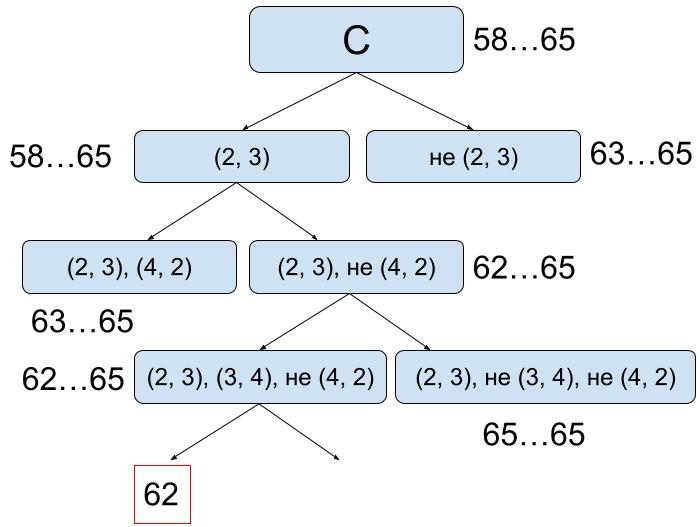
\includegraphics[scale=0.25]{result}}
\label{fig:image}
\end{figure}
\end{frame}

\begin{frame}
\frametitle{Пример: применение метода ветвей и границ на конкретной задаче}
Видно, что листов с нижней границей, меньшей 62, в дереве нет. Значит, найденный путь, обладая длиной 62, является ответом к задаче.
\end{frame}

\end{document}